\documentclass[12pt, letterpaper]{article}
\usepackage{listings}
\usepackage{graphicx}
\usepackage{color}
\usepackage{caption}
\usepackage{subcaption}
\usepackage{hyperref}
\usepackage{fancyhdr}
\usepackage{mathrsfs}
\usepackage[margin=3cm]{geometry}
\usepackage[dvips]{epsfig}
\usepackage{placeins}
\setlength{\parindent}{0.0in}
\setlength{\parskip}{0.05in}

\definecolor{dkgreen}{rgb}{0,0.6,0}
\definecolor{gray}{rgb}{0.5,0.5,0.5}
\definecolor{mauve}{rgb}{0.58,0,0.82}
\definecolor{deepblue}{rgb}{0,0,0.7}
\definecolor{deepred}{rgb}{0.6,0,0}
\definecolor{deepgreen}{rgb}{0,0.5,0}
\definecolor{red}{rgb}{0.9,0,0}

\newcommand\course{CS532}
\newcommand\semester{Spring 2017}
\newcommand\hwnum{3}
\newcommand\yourname{Justin Schaffner}
\newcommand\login{JASchaff}
\newenvironment{answer}[1]{\subsection*{Problem #1}}

\pagestyle{fancyplain}
\headheight 40pt
\lhead{\yourname\ (\login)\\\course\ --- \semester}
\chead{\textbf{\Large Assignment \hwnum}}
\rhead{\today}
\headsep 40pt
\lstnewenvironment{MyBash}{\lstset{language=bash, aboveskip=3mm, belowskip=3mm, showstringspaces=false, columns=flexible, basicstyle={\small\ttfamily}, numbers=none, numberstyle=\tiny\color{grey}, keywordstyle=\color{black}, commentstyle=\color{dkgreen}, stringstyle=\color{black}, breaklines=true, breakatwhitespace=true, tabsize=3}}{}
\lstnewenvironment{MyPython}{\lstset{language=Python, aboveskip=3mm, belowskip=3mm, basicstyle=\small, otherkeywords={self}, keywordstyle=\color{deepblue}, emph={MyClass,__init__}, emphstyle=\color{deepred}, stringstyle=\color{deepgreen}, commentstyle=\color{red}, frame=tb, showstringspaces=false, breaklines=true }}{}
\lstnewenvironment{MyR}{\lstset{language=R, aboveskip=3mm, belowskip=3mm, basicstyle=\small, breaklines=true}}{}

\begin{document}

\begin{answer}{1: Download and Parse HTML}
Eat\textunderscore HTML.py takes a text file of URLs as its only argument, pulls their HTML pages and saves them in a directory within the working directory called ``HTML\textunderscore pages\textbackslash ". If the directory does not exist, it makes a new directory. The name of each file is a hash of the URL using hashlib.sha224 plus the ``.html" extension. The filename and and the original URL are stored in the file ``hash\textunderscore table.txt" within the same directory. While running this program about 21 of the URLs raised an error, several while handling the gzip returned by the server. Most of these URL's were from Huffington Post. When tested with curl, they unpacked just fine. I also noticed that for an additional 23 URLS, while they returned ok, the resulting HTML was empty except for ``FORBIDDEN". There was a stack exchange post that said this was because in the GET request, the User Agent field is empty and some web pages don't like that. So I copied the User Agent from the header in Chrome on my laptop and that seemed to solve the issue. There were four links that still raised in error, but they all pulled a 301 error or could not resolve the host. I tried them all in curl and chrome. There were an additional 14 that resulted in an empty HTML file but they also were either broken links or the URL  returned ``finder.cox.net". Out of the 1025 URLs, 1007 were still usable.
 Here is the code for Eat\textunderscore HTML.py:
\begin{MyPython}
import hashlib
import requests
import os
from sys import argv
import bs4

class html_downloader():
    #converts URL to a filename ending in a provided extension
    def URL_to_filename(self, address, extension='.html'):
        m=hashlib.sha224(str(address).encode('utf-8')).hexdigest()
        filename=m.rstrip()+extension
        print(filename)
        return filename
    
    #pulls the page and processes it through process_page(tpage)
    def pull_page(self, address):
        address=address.rstrip()
        header={'User-Agent': 'Mozilla/5.0 (Macintosh; Intel Mac OS X 10_12_3) AppleWebKit/537.36 (KHTML, like Gecko) Chrome/56.0.2924.87 Safari/537.36'}
        tpage=requests.get(address, headers=header, allow_redirects=True)
        return tpage
        
    

if __name__ == '__main__':
    infilename=argv[1]
    h=html_downloader()
    filepath='HTML_pages/'
    directory=os.path.dirname(filepath)
    if not os.path.exists(directory):
        os.makedirs(directory)
    #a table with URLs and their hashed filenames
    with open('HTML_pages/hash_table.txt', 'a') as hashtable:
        #the list of URLs
        with open(infilename, 'r') as infile:
            for URL in infile:
                try:
                    tpage=h.pull_page(URL)
                    tname=h.URL_to_filename(URL, '.html')
                    hashtable.write(tname.rstrip()+'\t'+ URL)
                    tname=filepath.rstrip()+tname
                    tfile=open(tname, 'w')
                    tfile.write(tpage.text)
                except:
                    print('URL failed: ' + URL)
                    pass
\end{MyPython}
\FloatBarrier

For the second part of problem 1, parseing the HTML files, I made a second class called File\textunderscore Cruncher.py. Most of the functionality came directly from the stack exchange post mentioned in the assignment, with a few tweeks to make it work and using some of the suggestions from the comments.
Here is the code for File\textunderscore Cruncher.py:
\begin{MyPython}
from sys import argv
import bs4
import  os

class file_cruncher():
    #checks visibility of element
    def visible(self, element):
        if element.parent.name in ['style', 'script', '[document]', 'head', 'title', 'meta']:
            return False
        elif isinstance(element, bs4.element.Comment):
            return False
        return True
    #converts html file to txt file of visible text
    def de_HTML(self, filepath):
        soup=bs4.BeautifulSoup(open(filepath),'html.parser')
        texts=soup.find_all(text=True)
        visible_text=filter(self.visible, texts)
        newfilepath=os.path.join(os.path.dirname(filepath), (os.path.splitext(os.path.basename(filepath))[0].rstrip() + '.txt'))
        outfile=open(newfilepath, 'w')
        outfile.writelines('%s\n' % line for line in visible_text)
        outfile.close()
        
if __name__ == '__main__':
    directory=argv[1]
    fc=file_cruncher()
    for filename in os.listdir(directory):
        if filename.endswith('.html'):
            filepath=os.path.join(directory, filename)
            fc.de_HTML(filepath)
            print('Converted: ', filepath)
\end{MyPython}
\end{answer}
\begin{answer}{2: Search Directory and Corpus Analysis}
For this part I wrote two classes but put them together in one file, Search\textunderscore dir.py. It takes 3 arguments. The first is the directory you wish to search. The second is the search term, and the optional third is the number of results you want, with the default being 10. The first class, search\textunderscore dir(), has 3 functions. The first files\textunderscore contain() rummages through the directory passed to it, then calls the function meets() which uses mmap to check if the file contains the search term. Mmap was suggested in a stackexchange post as a low cost way of checking a large number of files for a term. The function files\textunderscore contain() returns a list of files containing the term. The third function uses the hash\textunderscore table.txt file to pull the priginal URL given the filename.txt. The second class corpus\textunderscore analysis() has two functions. The first calculates the TF (number of terms/number of words) and the second calculates the IDF(total corpus/number of results) by doing a google search. The size of the corpus is set to 30,000,000,000,000. I got that number from \url{http://www.statisticbrain.com/total-number-of-pages-indexed-by-google/}.
The data from the frist ten URLs returned with the search term 'gaga' gave the following table:
\begin{table}[!htbp]
\centering
\caption{10 hits for the term ``gaga" ranked by TFIDF}
\label{my-label}
\resizebox{\textwidth}{!}{%
\begin{tabular}{llll}
TF-IDF  & TF  & IDF  & URL\\
0.106  & 0.00409  & 26.0  & \url{http://worldofwonder.net/omgaga-official-lady-gaga-will-rupauls-drag-race-season-9/}\\
0.0829  & 0.00319  & 26.0  & \url{http://linkis.com/www.youtube.com/GFCPL}\\
0.0652  & 0.00251  & 26.0  & \url{http://www.elsalvador.com/articulo/famosos/lady-gaga-alquilo-lujosa-mansion-para-super-bowl-140280}\\
0.0605  & 0.00233  & 26.0  & \url{http://kroq.cbslocal.com/2017/02/07/lady-gaga-duet-metallica-grammys/}\\
0.0421  & 0.00162  & 26.0  & \url{http://metro.co.uk/2017/02/07/lady-gaga-and-metallica-to-perform-special-and-unique-duet-at-2017-grammy-awards-6433549/?ito=twitter}\\
0.0417  & 0.00161  & 26.0  & \url{http://www.metalinjection.net/shocking-revelations/metallica-to-perform-with-lady-gaga-at-the-grammys-this-weekend}\\
0.0415  & 0.0016  & 26.0  & \url{http://www.notiexpresscolor.com/2017/02/07/lady-gaga-engano-a-millones-con-falso-salto-video/}\\
0.0303  & 0.00117  & 26.0  & \url{http://www.instyle.com/news/lady-gaga-rupauls-drag-race-season-9-video?xid=soc_socialflow_twitter_instyle}\\
0.0229  & 0.000881  & 26.0  & \url{https://itunes.apple.com/gb/album/born-this-way/id903210172?ign-mpt=uo\%3D2}\\
0.0208  & 0.00080  & 26.0  & \url{https://www.youtube.com/watch?v=yk5RORfkeok}
\end{tabular}%
}
\end{table}
\newpage
Here is the code for Search\textunderscore dir.py:
\begin{MyPython}
import mmap
from sys import argv
import os
import requests
from bs4 import BeautifulSoup
import argparse
from math import log2, log10, floor
import re

#searches a directory for files containing a search term
class search_dir():
    def files_contain(self, directory, search_term):
        file_list=[]
        empty_file=0
        total_file=0
        for filename in os.listdir(directory):
            try:
                if filename.endswith('.txt') and not filename.startswith('hash'):
                    print(filename)
                    filepath=os.path.join(directory, filename)
                    total_file+=1
                    if self.meets(filepath, search_term):
                        file_list.append(filepath)
            except:
                empty_file+=1
                URL=self.get_orig_URL( (os.path.splitext(filename)[0].rstrip() + '.html'), os.path.join(directory, 'hash_table.txt'))
                print('Empty File count: ', empty_file, '\tUsable File count: ', total_file-empty_file, '\nURL: ', URL)
                pass
        print('Empty File count: ', empty_file, '\tUsable File count: ', total_file-empty_file)
        return file_list
                    
    def meets(self, filepath, search_term):
        with open(filepath, 'r+b', 0) as file, \
             mmap.mmap(file.fileno(), 0, access=mmap.ACCESS_READ) as s:
            if s.find(bytes(search_term, 'utf-8')) != -1:
                return True
            return False
    def get_orig_URL(self, filename, hash_table_file_path):
        with open(hash_table_file_path, 'r') as hash_file:
            #print('search for: ', filename)
            for line in hash_file:
                fields=line.split('\t')
                if fields[0]== filename:
                    return fields[1]
            return 'oops'
               
#analyzes a stripped html file for TF = #search_term/#words
#and also searches google for search term and returns IDF=search_results/size_of_index                     
class corpus_analysis():
    def get_TF(self, filepath, search_term):
        term_count=0
        word_count=0
        with open(filepath, 'r') as file:
            for line in file:
                words=line.split()#re.findall('[a-zA-Z_]+',line)
                word_count+=len(words)
                for i in words:
                    if search_term in i:
                        term_count+=1
            return term_count/word_count

    def get_IDF(self, search_term):
        #this number came from http://www.statisticbrain.com/total-number-of-pages-indexed-by-google/
        google_index=30000000000000
        parser = argparse.ArgumentParser(description='Get Google Count.')
        parser.add_argument('--word', help='word to count')
        args = parser.parse_args(['--word=search_term'])
        #pulls the google search results
        r = requests.get('http://www.google.com/search',
                         params={'q':'"'+args.word+'"',
                                 "tbs":"li:1"}
                        )

        soup = BeautifulSoup(r.text, "lxml")
        line= soup.find('div',{'id':'resultStats'}).text
        line=line.replace(',','')
        results=int(re.search(r'\d+', line).group())
        print ('Google Search Results: ', results)
        return log2(google_index/results)

#arg 1 directory arg 2 search term arg 3 number of results wanted(default is 10)
if __name__ == '__main__':
    directory=argv[1]
    search_term=argv[2]
    if len(argv)>3:
        count=argv[3]
    else:
        count=10
    search=search_dir()
    CA= corpus_analysis()
    #searches directory for matching txt files excluding hash table
    file_list=search.files_contain(directory, search_term)
    #gets the TF and IDF and TF-IDF for each file and stores it in a list
    results_list=[]
    round_to_n=lambda x, n: round(x, -int(floor(log10(abs(x))))+(n-1))
    IDF=CA.get_IDF(search_term)
    rIDF=round_to_n(IDF, 3)
    print('IDF: ', IDF)
    for filepath in file_list[:count]:
        print(filepath)
        TF=CA.get_TF(filepath, search_term)
        print('TF: ',TF)
        TF_IDF=TF * IDF
        TF=round_to_n(TF, 3)
        TF_IDF=round_to_n(TF_IDF, 3)
        URL=search.get_orig_URL( (os.path.splitext(os.path.basename(filepath))[0].rstrip() + '.html'), os.path.join(directory, 'hash_table.txt'))
        results_list.append([TF_IDF, TF, rIDF, URL])
    with open('TF_IDF_results.txt', 'w') as outresults:
        print('TF-IDF', 'TF', 'IDF', 'URL', sep='\t', end='\n', file=outresults)
        for result in results_list:
            print(*result, sep='\t', file=outresults)
\end{MyPython}
\end{answer}
\begin{answer}{3: Page Rank}
For the page rank, I used the first page rank page suggested in the assignent \url{http://pr.eyedomain.com/} and got the following results:\\
\FloatBarrier
\begin{table}[!htbp]
\centering
\caption{10 hits for the term ``gaga" ranked by Page Rank}
\label{my-label}
\resizebox{\textwidth}{!}{%
\begin{tabular}{ll}
Page Rank  & URL\\
0.9  & \url{https://www.youtube.com/watch?v=yk5RORfkeok}\\
0.9  & \url{https://itunes.apple.com/gb/album/born-this-way/id903210172?ign-mpt=uo\%3D2}\\
0.7  & \url{http://www.instyle.com/news/lady-gaga-rupauls-drag-race-season-9-video?xid=soc_socialflow_twitter_instyle}\\
0.7 & \url{http://kroq.cbslocal.com/2017/02/07/lady-gaga-duet-metallica-grammys/}\\
0.6 & \url{http://metro.co.uk/2017/02/07/lady-gaga-and-metallica-to-perform-special-and-unique-duet-at-2017-grammy-awards-6433549/?ito=twitter}\\
0.6 & \url{http://www.elsalvador.com/articulo/famosos/lady-gaga-alquilo-lujosa-mansion-para-super-bowl-140280}\\
0.5 & \url{http://www.metalinjection.net/shocking-revelations/metallica-to-perform-with-lady-gaga-at-the-grammys-this-weekend}\\
0.5  & \url{http://worldofwonder.net/omgaga-official-lady-gaga-will-rupauls-drag-race-season-9/}\\
NA & \url{http://www.notiexpresscolor.com/2017/02/07/lady-gaga-engano-a-millones-con-falso-salto-video/}\\
NA  & \url{http://linkis.com/www.youtube.com/GFCPL}\\
\end{tabular}%
}
\end{table}
\FloatBarrier
Two of the URLs had no Page Rank. The second one, linkis.com, looks like a click bait page. The second might be a Spanish news site. For the TFIDF, linkis.com actually had the second highest rank. When I looked at the text file for this page after it had been parsed, the number of words was really low compared to other pages, while Gaga is mentioned several times. The Spanish newsite mentioned Gaga more, but it had a higher word count, coming in 7th. iTunes actually came very low on the TFIDF, since it had a high wordcount and only mentioned Gaga by name a few times, since most of her songs don't have her name in the title, but obviously their Page Rank was one of the highest. If I was searching for Gaga, its more likely that I want to see her music or a legitimate news article than a video about how Satan is speaking through her to take dominion of the Earth, which is what linkis.com takes you to.
\end{answer}
\begin{answer}{4: Tau-b}
When comparing the data in Table 1 for TFIDF to the PageRank data in table 2, you can find the level of correlation using Kendall's Tau-b formula. Table 3 shows the comparison of that data with concordant and discordant values.
\FloatBarrier
\begin{table}[!htbp]
\centering
\caption{Concordant and Discordant pairs}
\label{my-label}
\begin{tabular}{llllll}
URL  & Page Rank  & TFIDF  & C  & D\\
youttube  & 0.9  & 0.0208  & 0  & 9\\
itunes  & 0.9  & 0.0229  & 0  & 8\\
instyle  & 0.7  & 0.0303  & 0  & 7\\
kroq  & 0.7 & 0.0605  & 3  & 3\\
metro  & 0.6 & 0.0421  & 2  & 3\\
elsalvador  & 0.6 & 0.0652  & 2  & 2\\
metalinjection  & 0.5 & 0.0417  & 1  & 2\\
worldofwonder  & 0.5  & 0.106  & 2  & 0\\
natiexpress  & 0.0  & 0.0415  & 0  & 1\\
linkis  & 0.0  & 0.829\\
& & Total  & 10  & 35
\end{tabular}
\end{table}
\FloatBarrier
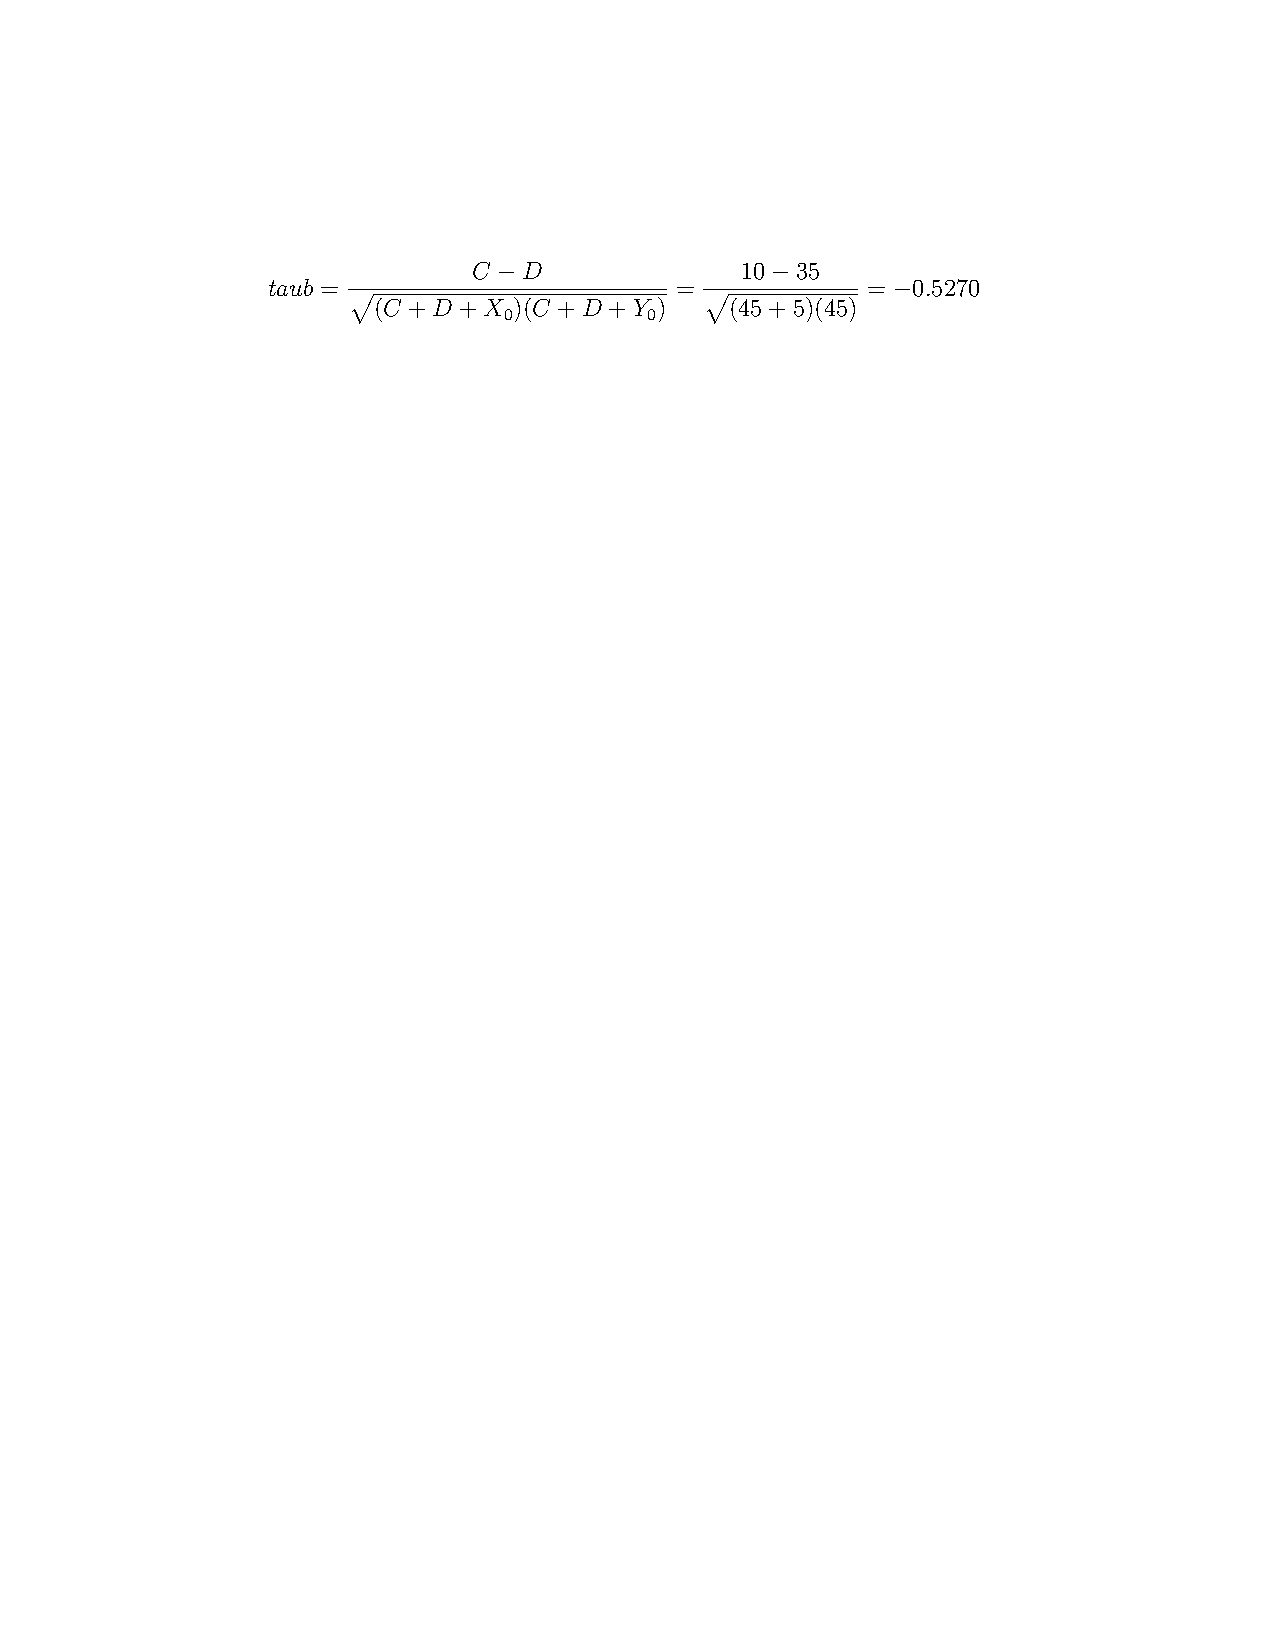
\includegraphics[width=\linewidth]{Tau_b}\\
Where C is the total concordant pairs, D is the total discordant pairs, X\textsubscript{0} is the number of ties in Page Rank and Y\textsubscript{0} is the same for TF-IDF. \\
For the p-value I used the Z\textsubscript{b} equation from wikipedia.\\
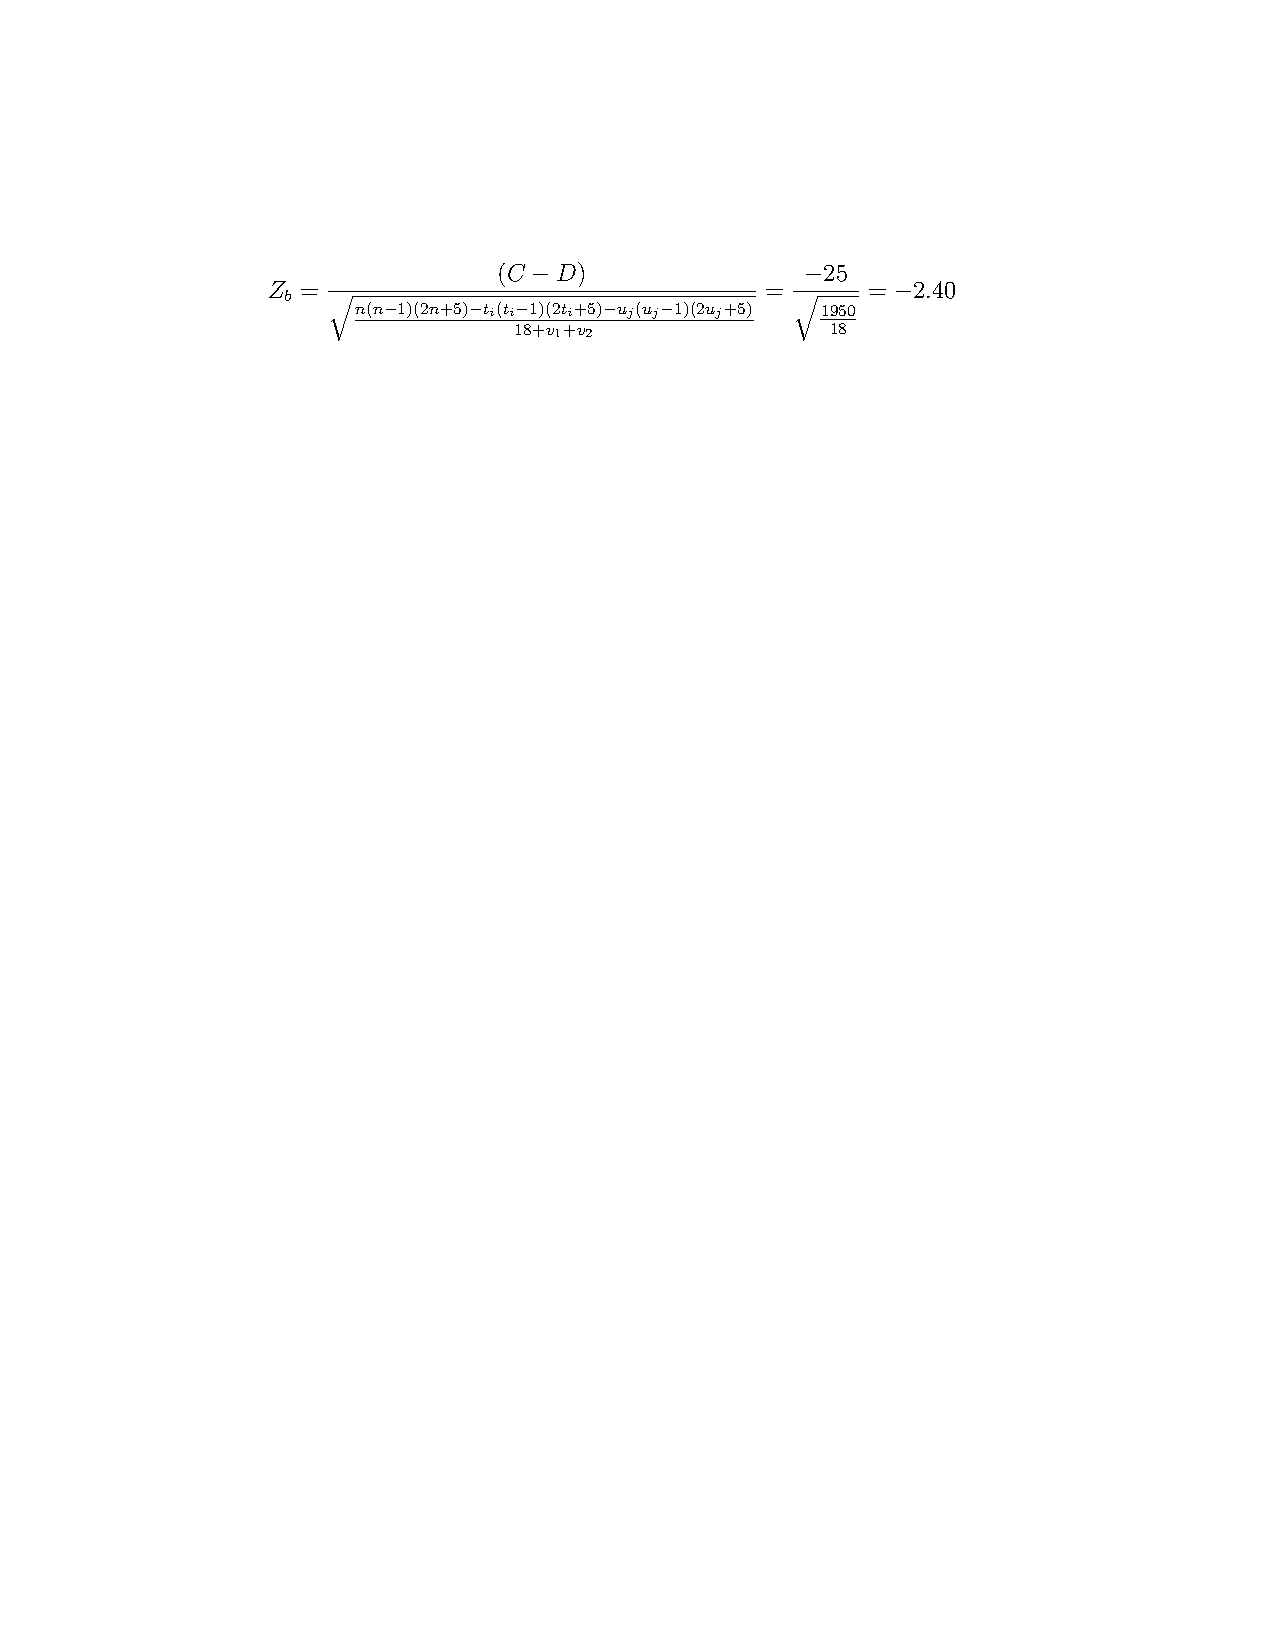
\includegraphics[width=\linewidth]{Zed_b}\\
I compared -2.40 to a Z table I found at \url{http://www.statisticshowto.com/tables/z-table/} and got a p value of 0.4918. When added with the right side I got: \\
\centerline{
\includegraphics[width=.5\linewidth]{p_value}}\\
The p-value would suggest that there is little correlation between the Page Rank and TFIDF that I calculated. 
\end{answer}
\end{document}